\section{Experiments}\label{sec:experiments}

\begin{figure*}[!t]
  \centering
  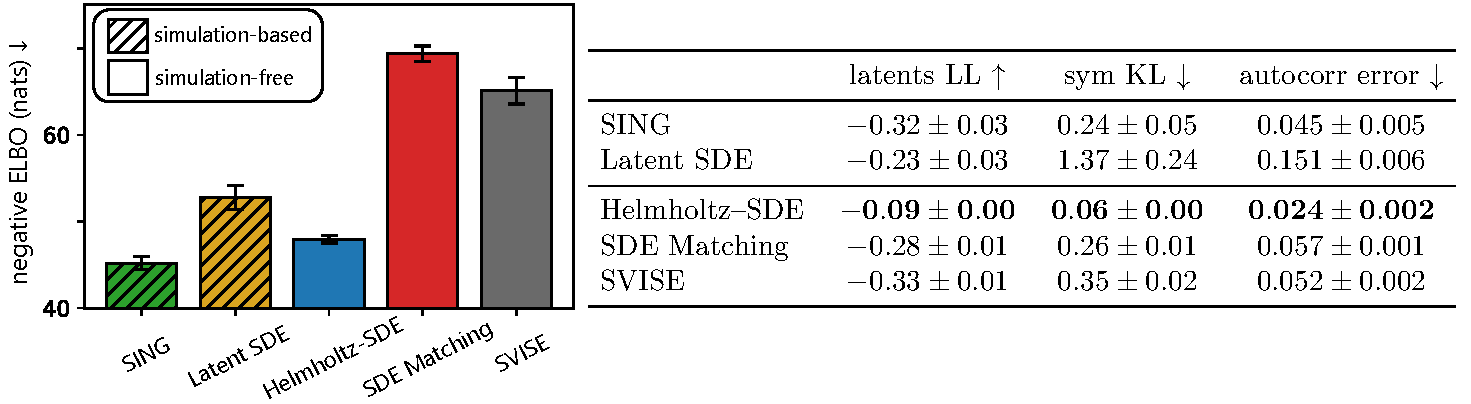
\includegraphics[width=\textwidth]{figs/fig_x.pdf}

    \caption{Helmholtz-SDE closes the gap between simulation-based and simulation-free VI algorithms on the noisy Lorenz attractor. Negative ELBO and LL of true latents under the posterior are averaged over trials; sym KL is averaged over one-time marginals. Autocorr error is the entrywise RMSE of the global $3{\times}3$ autocorrelation matrix, averaged over horizon $t{=}2$. Errors are $\pm2$SE over 10 replicates.}
  \label{fig:lorenz}
  \vspace{-1em}
\end{figure*}

We validate experimentally that Helmholtz-SDE shrinks the expressivity gap between simulation-free and simulation-based VI, with downstream improvements in dynamics learning. 
We begin with a linear, conjugate setting where the posterior is tractable and the gap can be quantified directly (\Cref{subsec:ou}), then move to nonlinear synthetic dynamics (\Cref{subsec:lorenz}) and two real-world systems: predator-prey cycles (\Cref{subsec:predator-prey}) and reduced order fluid dynamics (\Cref{subsec:rom}).

Throughout, we match implementation choices across methods.
In particular, existing VI algorithms differ in how they amortize the posterior approximation: across time, by representing it as a function of $t$, and across trials, by using an encoder to produce trial-specific parameters. 
Both strategies reduce memory at some cost to expressivity. 
We use the same amortization scheme whenever a method supports it.
For Helmholtz-SDE we use the degree $\ell =1$ polynomial approximation in all experiments; we provide ablations of the polynomial degree in \Cref{app:sec:nonlinear-sde}.
Full experimental details are in \Cref{app:sec:ou-spiral,app:sec:nonlinear-sde}.
We provide runtime comparisons against all baselines in \Cref{app:sec:timing}.

\subsection{Ornstein-Uhlenbeck (OU) spiral}\label{subsec:ou}
We first study the impact of augmenting the variational family in the conjugate setting, where the suboptimality of both the variational posterior and the learned prior can be analyzed directly. We consider the two-dimensional OU spiral
\begin{equation}
\label{eqn:ou-spiral}
    \bbP\!: \; d \mbx(t) = (-\alpha \bbI_2 + \omega \mbJ)\mbx(t)dt + d\mbw(t), 
    \quad
    p(\mbx,0) = \cN\left(\mb0, \tfrac{1}{2\alpha}\bbI_2\right),
    \quad
    \mbJ = \bigl(\begin{smallmatrix} 0 & -1 \\ 1 & 0 \end{smallmatrix}\bigr)
\end{equation}
whose drift decomposes into a contracting gradient field $-\alpha \mbx$ and a $p$-divergence-free rotational field $\omega \mbJ \mbx$. Observations follow the linear-Gaussian model $p(\mby(t_i) | \mbx(t_i)) = \cN(\mbC\mbx(t_i)+\mbd, \sigma^2 \mbC\mbC^\top)$.

\paragraph{Suboptimality of inference.}
\Cref{thm:helm-optimal} establishes that Helmholtz-SDE has zero KL gap to the posterior in this setting. In \Cref{app:subsec:ou-theory}, we show that the choices of variational drift made by SDE Matching \cite{bartosh2025sde} and SVISE \cite{course2023state,course2023amortized}, which we refer to as the ``square root'' and  ``symmetric'' gauges, respectively, incur a KL gap that grows linearly in $\omega$. We validate this in simulation. Fixing $T_{\max} = 5$ and $\alpha = 0.2$, we vary observation noise $\sigma$, number of observations $N$, and rotational speed $\omega$. 
\Cref{fig:spiral-results}A shows that when prior rotation is strong, Helmholtz-SDE achieves a variational approximation orders of magnitude closer in symmetric KL to the true posterior than the square root gauge, with the largest gains at sparse observations and large noise. 
When $\omega = 0$ (\Cref{fig:spiral-zero}), the posterior drift contains no divergence-free component, in which case the square root gauge can represent it exactly. 
Results for the symmetric gauge and $\omega \in \{\pi/4, \pi/2, \pi\}$ are in \Cref{app:subsec:ou-spiral-supplement}.

\paragraph{Degradation in learning.}
We next test whether posterior misspecification degrades learning. 
Using the same grid of $(\sigma, N, \omega)$ values, we jointly learn the prior (parameterized by a neural network drift) and observation model from $1024$ independent trials. 
\Cref{fig:spiral-results}B and D show that the regimes where the square root gauge yields the worst posterior approximation are also where prior learning degrades most. 
In many cases, the divergence-free correction is the difference between recovering the correct drift and learning an incorrect one (\Cref{fig:spiral-results}C).
However, consistent with previous work \cite{turner2011two}, better variational approximations do not translate monotonically to improvements in learning.

\begin{figure*}[!t]
  \centering
  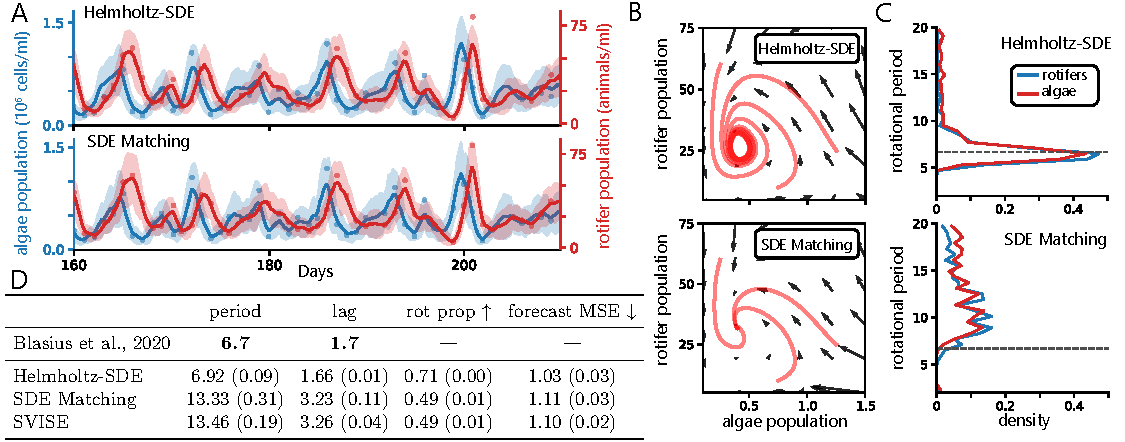
\includegraphics[width=\textwidth]{figs/fig3-rotifer-algae.pdf}
  \caption{Helmholtz-SDE recovers predator-prey dynamics more faithfully than SDE Matching. \textbf{A}: Posterior mean $\pm 2$ SD over a representative window. 
  \textbf{B}: Phase portraits of learned dynamics: Helmholtz-SDE recovers a limit cycle, SDE Matching decays to a fixed point. 
  \textbf{C}: Peak-period distribution across 100-day forward simulations from the learned prior; dashed line marks the empirical period of 6.7 days.
  \textbf{D}: Rotation period, predator lag, and proportion of time in coherent rotation computed per replicate as the median across forward simulations using the wavelet analysis of \citet{blasius2020long}; forecast MSE, in log coordinates. 
  Values are median (IQR) across 10 replicates.
 }
  \label{fig:rotifer-algae}
  \vspace{-1em}
\end{figure*}

\subsection{Noisy Lorenz attractor}\label{subsec:lorenz}

In the following three subsections, we demonstrate that the advantages from \Cref{subsec:ou} extend to nonlinear dynamics. 
We first consider Lorenz attractor dynamics, a classical chaotic system. 
The standard setup of \citet{li2020scalable} uses small process noise and dense, low-noise observations; in this regime the posterior concentrates tightly around the true latent trajectory (\Cref{fig:lorenz-compare}A). 
To simulate a setting with non-trivial posterior uncertainty, we sample latents on $[0, 5]$ with increased process noise and observe them every $\Delta t = 0.25$ (\Cref{fig:lorenz-compare}B). 
We perform joint inference and learning using $1024$ trials with $K{=}4$ latent dimensions, evaluating both one-time (symmetric KL to the true prior) and multi-time (lagged autocorrelation error) statistics of the prior.

We compare Helmholtz-SDE to simulation-free (SDE Matching \cite{bartosh2025sde}, SVISE \cite{course2023state,course2023amortized}) and simulation-based (SING \cite{hu2025sing}, Latent SDE \cite{li2020scalable}) baselines (\Cref{fig:lorenz}). 
Among simulation-free methods, Helmholtz-SDE achieves a ${\sim}20$\,nat smaller negative ELBO than the alternatives, reflecting the inability of a pre-specified drift to represent the posterior path law. 
As a result, only Helmholtz-SDE accurately learns the outward-spiraling dynamics within each lobe of the attractor (\Cref{fig:lorenz-samples}). 
Helmholtz-SDE also matches or exceeds simulation-based methods in dynamics recovery. 
SING attains a slightly tighter nELBO but at substantially higher cost: on an H100 GPU, Helmholtz-SDE reaches per-trial nELBO below $50$\,nat in $123.7 \pm 3.4$\,s, whereas SING requires $3695.6 \pm 503.8$\,s, over $25\times$ slower.

\subsection{Predator-prey system}\label{subsec:predator-prey}
Predator-prey systems exhibit cyclic dynamics in which the predator population lags the prey, and recovering this lag structure is important to ecological interpretation \cite{lotka1925elements,volterra1926fluctuations,elton1942ten,utida1957cyclic,berryman2002population}.
Because the lag is a multi-time statistic, it directly probes the path law approximation made by simulation-free algorithms.

We study the dataset of \citet{blasius2020long}, who cultivate rotifers (\textit{B.~calyciflorus}, a freshwater zooplankton) feeding on algae in a controlled environment and measure both populations daily for up to 374 days. 
The system exhibits persistent cycles with a mean period of 6.7 days, in which the rotifer population lags the algae by approximately 1.7 days. 
Rather than imposing a biological model on dynamics \cite{mccauley1996structured}, we aim to learn a generative model of the dynamics directly from data.

To this end, we consider the longest trial and restrict to windows of coherent oscillation following \citet{blasius2020long}, yielding $255$ days of data across $4$ subtrials. We hold out the last $8$ days of each (${\sim}1$ cycle) for forecasting. 
We then fit Helmholtz-SDE, SDE Matching, and SVISE on the log-transformed rotifer and algae populations with $K{=}2$ latent dimensions. 

All methods produce plausible posterior approximations over the observed populations (\Cref{fig:rotifer-algae}A).
However, the learned generative dynamics differ qualitatively: Helmholtz-SDE yields a stable limit cycle, while SDE Matching decays to a fixed point (\Cref{fig:rotifer-algae}B).
Moreover, the rotational dynamics learned by Helmholtz-SDE closely match the true biological system, with median period $6.92$ days and predator-prey lag $1.66$ days, both close to the estimates from \citet{blasius2020long} (\Cref{fig:rotifer-algae}C,D). 
SDE Matching, in contrast, recovers a period twice as long ($13.33$ days) and a correspondingly inflated lag ($3.23$ days). 
We provide details on our wavelet analysis in \Cref{app:subsec:predator-prey}.

\subsection{Reduced order models of fluid dynamics}\label{subsec:rom}

\begin{figure*}[!t]
  \centering
  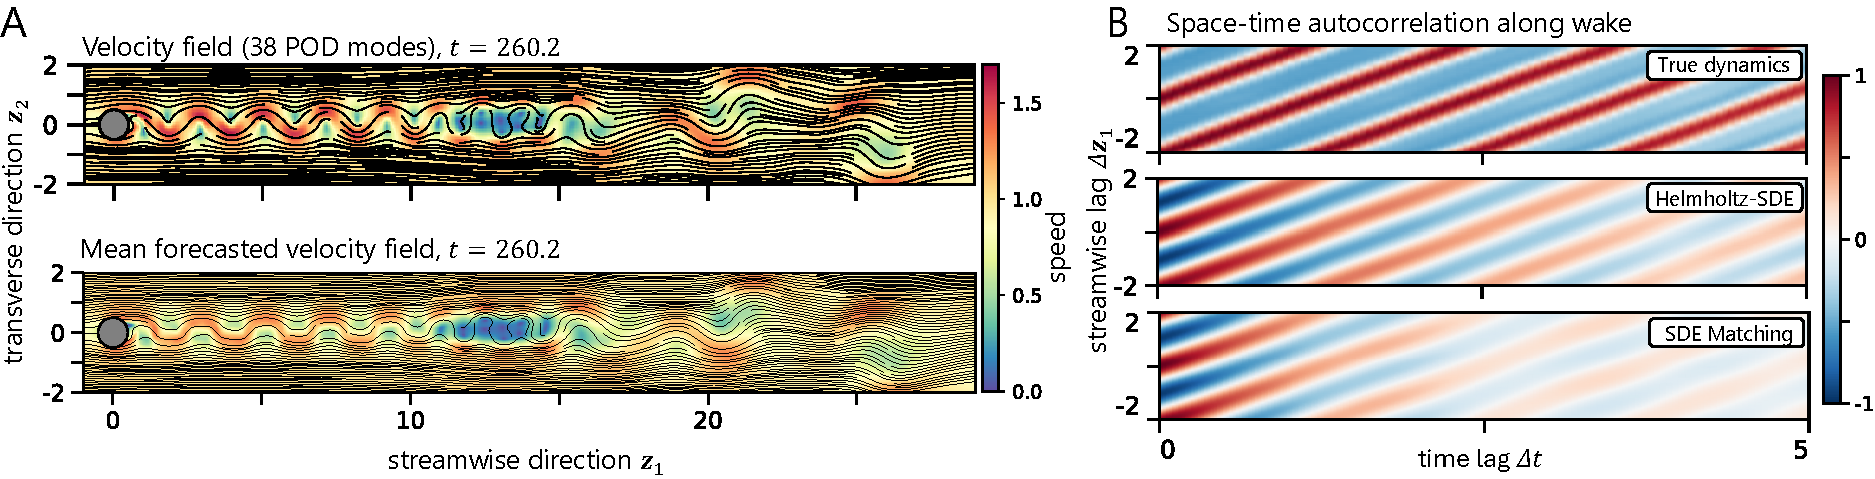
\includegraphics[width=\textwidth]{figs/fig4-2d-cylinder.pdf}
    \caption{
    Helmholtz-SDE learns coherent wake dynamics in high-dimensional fluid flow past a 2D cylinder.
    \textbf{A}: True and forecasted mean velocity fields at $4$ time units into the forecast window.
    \textbf{B}: Joint space–time autocorrelation along the streamwise direction in the vortex region $[1, 10] \times [-0.1, 0.1]$, from prior samples at the true $t{=}0$ initial condition.
    Diagonal banding indicates vortices being advected downstream at a coherent speed; rapid decay reflects loss of temporal coherence. 
    }
  \label{fig:fluid-dynamics}
  \vspace{-1.5em}
\end{figure*}

As a final case study, we apply Helmholtz-SDE to a problem in computational fluid dynamics: modeling a two-dimensional incompressible flow past a circular cylinder at Reynolds number $2 \cdot 10^3$, a regime with strong, persistent vortices in the wake (\Cref{fig:fluid-dynamics}A). 
We use the dataset of \citet{course2023state}, in which the Navier--Stokes equations are discretized and solved on a grid of nearly $6 \cdot 10^5$ points using the immersed boundary projection method \cite{taira2007immersed}.


Reduced order modeling (ROM) provides a toolkit for representing such high-dimensional systems with low-dimensional surrogates. 
Classical projection-based approaches require explicit access to the discretized PDE \cite{brunton2020machine}.
Data-driven approaches instead learn reduced dynamics directly from snapshots of the time series, sidestepping projection of the PDE.
Following \citet{course2023state}, we apply dimensionality reduction (POD, \cite{sirovich1987turbulence, berkooz1993proper}) to velocity snapshots and retain $K = 38$ modes capturing $90\%$ of the kinetic energy.
We observe each POD coefficient, perturbed by Gaussian noise, every $\Delta t = 0.3$ time units over an interval of length $195.2$. 
We hold out $10$ time units for forecasting.

Helmholtz-SDE successfully learns a ROM of the cylinder dynamics (\Cref{fig:fluid-dynamics}A).
The space--time autocorrelation along the wake reveals that, compared to SDE Matching, Helmholtz-SDE better recovers the traveling-wave structure of vortex advection (\Cref{fig:fluid-dynamics}B). 
This translates to an approximately $10\%$ reduction in integrated MSE over SDE Matching and SVISE over the 10-unit forecast window, at modest additional training cost (approx.~3$\times$ larger per-iteration cost on H100 GPU). 
This example demonstrates that even for moderate latent dimensions $K$, our approximation to the Helmholtz decomposition remains tractable and yields improvements in dynamics learning.